\documentclass[a4paper,12pt,oneside]{report}
\usepackage[final]{listings}
\usepackage{url}
\lstset{breaklines=true}
\usepackage{graphicx}
\graphicspath{ {images/} }
\setcounter{tocdepth}{4}
\hbadness=5000
\begin{document}
\title{
{ Implementing and Developing Geo-visualization techniques showing the large amount of historical and geospatial and temporal data available in the Linked Open Data Cloud on a specific example }\\
{
\includegraphics{university.png}}}
\author{Abderrahmen Sdiri}
\date{\today}
\maketitle
\chapter*{Abstract}
{The project aims to investigate geo-visualization techniques showing a large amount of historical ,geospatial and temporal data available in the Linked Open Data Cloud: http://lod-cloud.net/ and other open data sources . We selected the example of Belgium, we focused on :Population ,external immigration and number of  crimes  in the 3 regions of Belgium(Flemish,Walloon,Brussels-Capital) and we tried to find a  correlation between those datasets to understand the causes of the crimes in Belgium .The data are gathered, processed ,converted to linked data  and visualized .The data  can be accessed by authorized users over the Internet using an intuitive graphical user interface (GUI) to be implemented. The visualization can be beneficial for understanding the impact of the different factors affecting changes.}
\pagenumbering{roman}
\chapter*{Dedication}
\chapter*{Acknowledgements}
\tableofcontents
\listoffigures
\listoftables
\newpage
\pagenumbering{arabic}
 \chapter*{General introduction}
{Nowadays, there are many techniques of processing data. Unfortunately, there are many different data formats one can work with. It makes the processing a lotmore difficult. The task becomes even harder when one wants to connect two different datasets in order to benefit from the connection. The connection allows us to get some additional information about entities from each of the standalone datasets. Therefore, a lot of computation time is spent on converting, formatting and transforming data into another form. But transforming datasets into
a matching format is not enough. One needs to specify how the data should be linked together.There are many ways of doing that. Starting with implementing the logic into a simple conversion script according to a specific dataset to introducing a more complex metadata description framework for purposes of generic data processing. Since one of the most attractive tasks in this area is to be able to connect any of the datasets available on the Internet, we are interested in the generic description frameworks. We would like to have a tool, which enables us to work with any data on the Internet formatted according to some kind of rules. We would like to link them together, analyze them and visualize them.
One of the most used description frameworks is the Resource Description Framework . It is a standard model for data interchange on the Web. It tells us how to describe resources on the Internet in order to allow other people, applications and tools to understand such a description. That gives us a potentialto link any data on the Internet. Based on the framework, a new model named Linked Data was introduced. The model has been brought up to make data interconnecting easier.
The result of interconnecting data while utilizing the principles of the Linked Data model and Resource Description Framework is a directed graph. Its vertices represent resources we have information about. The edges stand for relations between such entities. From this point on, it is up to us, how we look at the data. We can either explore them in a plain graph or apply some more semantics and make domain specific visualizations while using ontologies and other advanced techniques.One of the specific domains are statistical data, which are one of the most interesting kind of data. They are produced and processed by many stakeholders. In the context of Linked Open Data, the most interesting are, of course,governments and scientific groups. But we would like to work with such data in the usual way — make tables, charts or more interesting visualizations. }

In section \ref{sec:sem}, we look at the semantic web.

\chapter{Data science}
\textbf{\large Introduction}\\ \\
{In this chapter, we make an overview of data science by explaining the main idea behind it and its main purpose. We will also  present its activities .Besides ,we will focus  on data analysis part  which is among basic concepts of this work. The benefits of data analysis will be set in the end of this chapter.}
\section{Data science}
\subsection{Overview}
{  Data Science is the art of turning data into actions. This is accomplished through the creation of data products, which provide actionable information without exposing decision makers to the underlying data or analytics (e.g. buy/sell strategies for financial instruments, a set of actions to improve product yield, or steps to improve product marketing). A data product is produced from a statistical analysis. Data products automate complex analysis tasks or use technology to extend the usefulness of informal data model, algorithmic or inference.
Performing Data Science requires the extraction of timely, actionable information from diverse data sources to drive data products.
Examples of data products include answers to questions such as:
“Which of my products should I advertise more heavily to increase profit? How can I improve my compliance program, while reducing costs? What manufacturing process change will allow me to build a better product?” The key to answering these questions is: understand the data you have and what the data inductively tells you.
Data scientists use their data and analytical ability to find and interpret rich data sources, manage large amounts of data despite hardware, software, and bandwidth constraints.They merge also data sources and ensure consistency of datasets, moreover data scientists  create visualizations to aid in understanding data.In addition they build mathematical models using the data and present and communicate the data insights/findings. They are often expected to produce answers in days rather than months, work by exploratory analysis and rapid iteration, and to produce and present results with dashboards (displays of current values) rather than papers/reports, as statisticians normally do.}
\subsection{Data Science Activities }
{Data Science is a complex field. It is difficult, intellectually taxing work, which requires the sophisticated integration of talent, tools and techniques. But we need to cut through the complexity and provide a clear, yet effective way to understand this new world. To do this, we will transform the field Data Science into a set of simplified activities a, The Four Key Activities of a Data Science Endeavor.
\begin{enumerate}
\item \textbf {To acquire:} {This activity focuses on obtaining the data you need. Given the nature of data, the details of this activity depend heavily on who you are and what you do. As a result, we will not spend a lot of time on this activity other than to emphasize its importance and to encourage an expansive view onwhich data can and should be used.}
\item \textbf {To prepare:} {Great outcomes don’t just happen by themselves. A lot depends on preparation, and in Data Science, that means manipulating the data to fit your analytic needs.
This stage can consume a great deal of time, but it is an excellent investment. The benefits are immediate and long term.}
\item \textbf {To analyse: }{This is the activity that consumes the lion’s share of the team’s attention.
It is also the most challenging and exciting (you will see a lot of ‘aha moments’ occur in this space). As the most challenging and vexing of the four activities, this field guide focuses on helping you do this better and faster.}
\item \textbf {To Act:} {Every effective Data Science team analyzes its data with a purpose – that is, to turn data into actions. Actionable and impactful insights are the holy grail of Data Science.
Converting insights into action can be a politically charged activity, however. This activity depends heavily on the culture and character of your organization, so we will leave you to figure out those details for yourself.}
\end{enumerate}
\begin{figure}[ht]
\centering
\includegraphics[width=1\textwidth]{"Data science activities"}
\caption{Data science activities}
\end{figure}
\section{Data analysis}
\subsection{Definition}
{      The term “data analysis” refers to the process by which large amounts of raw data is reviewed in order to determine conclusions based on that data. It is the process of bringing order, structure and meaning to the mass of collected data. The data is often unorganized, and may come from different sources.Analysis of data is a process of inspecting, cleaning, transforming, and modeling data with the goal of discovering useful information, suggesting conclusions, and supporting decision-making. Data analysis has multiple facets and approaches, encompassing diverse techniques under a variety of names, in different business, science, and social science domains.The nature of data analysis varies, and correlates to the type of data being examined. For example, a business may concentrate on things such as determining employee performance, sales performance by department or sales person, etc. An economist, however, might look for identifiable patterns that explain the spending habits of various consumers.}
\subsection{Types of data analysis }
{     There are many different types of data analysis, all geared towards the nature of the data being analyzed. Generally speaking there are two broad categories: “quantitative analysis” and “qualitative analysis”}
\subsubsection{Qualitative Analysis}
{    Qualitative analysis deals with the analysis of data that is categorical in nature. In other words, data is not described through numerical values, but rather by some sort of descriptive context such as text. Data can be gathered by many methods such as interviews, videos and audio recordings, field notes, etc.
Once data is gathered it then needs to be interpreted. Often times this involves “coding”, which refers to the grouping of data into identifiable themes. Themes are then given a unique “label”, and each label can then be quickly grouped and contrasted to each other.Of course data must also be interpreted. Interpretation can be a part of the coding process, but this is not always the case.Qualitative analysis can be summarized by three basic principles (Seidel, 1998):
Notice things, Collect things, Think about things}
\subsubsection{Quantitative Analysis}
{   Quantitative analysis refers to the process by which numerical data is analyzed, and often involves descriptive statistics such as mean, media, standard deviation, etc. An in-depth discussion of quantitative analysis is beyond the scope of this article. Generally speaking, however, the following are often involved with quantitative analysis:
Statistical models, Analysis of variables, Data dispersion, Analysis of relationships between variables, Contingence and correlation, Regression analysis, Statistical significance, Precision Error limits}
\begin{table}
\begin{center}
\begin{tabular}{|c|c|}
\hline
Qualitative Data & Quantitative Data\\
\hline
Data is observed  & Data is measured \\
\hline
Involves descriptions& Involves numbers \\
\hline
Emphasis is on quality&Emphasis is on quantity\\
\hline
Examples are color, smell, taste&Examples are volume, weight, etc.\\
\hline
\end{tabular}
\end{center}
\caption{Comparison of Qualitative and Quantitative Analysis}
\end{table}
\subsection{The process of data analysis }
{Analysis refers to breaking a whole into its separate components for individual examination. Data analysis is a process for obtaining raw data and converting it into information useful for decision-making by users. Data is collected and analyzed to answer questions, test hypotheses or disprove theories.
Statistician John Tukey defined data analysis in 1961 as: "Procedures for analyzing data, techniques for interpreting the results of such procedures, ways of planning the gathering of data to make its analysis easier, more precise or more accurate, and all the machinery and results of (mathematical) statistics which apply to analyzing data. "
There are several phases that can be distinguished, described below. The phases are iterative, in that feedback from later phases may result in additional work in earlier phases.}
\begin{figure}[ht]
\centering
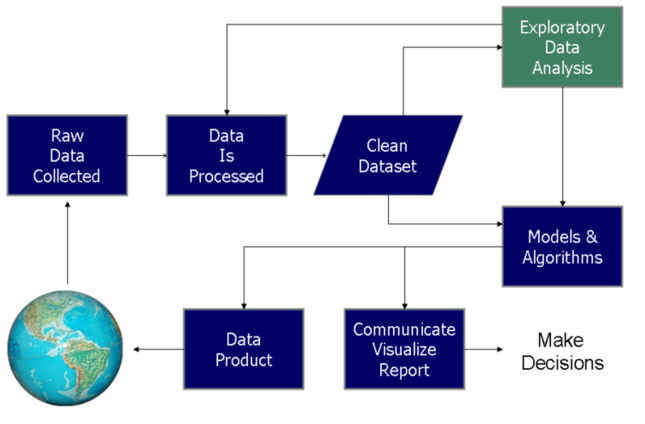
\includegraphics[width=1\textwidth]{Capture2}
\caption{The process of data science}
\end{figure}
\subsubsection{Data requirements}
{The data necessary as inputs to the analysis are specified based upon the requirements of those directing the analysis or customers who will use the finished product of the analysis. The general type of entity upon which the data will be collected is referred to as an experimental unit (e.g. a person or population of people). Specific variables regarding a population (e.g., age and income) may be specified and obtained. Data may be numerical or categorical (i.e., a text label for numbers).}
\subsubsection{Data collection}
{Data is collected from a variety of sources. The requirements may be communicated by analysts to custodians of the data, such as information technology personnel within an organization. The data may also be collected from sensors in the environment, such as traffic cameras, satellites, recording devices, etc. It may also be obtained through interviews, downloads from online sources, or reading documentation.}
\subsubsection{Data processing}
{The phases of the intelligence cycle used to convert raw information into actionable intelligence or knowledge are conceptually similar to the phases in data analysis.
Data initially obtained must be processed or organized for analysis. For instance, this may involve placing data into rows and columns in a table format for further analysis, such as within a spreadsheet or statistical software.}
\subsubsection{Data cleaning}
{Once processed and organized, the data may be incomplete, contain duplicates, or contain errors. The need for data cleaning will arise from problems in the way that data is entered and stored. Data cleaning is the process of preventing and correcting these errors. Common tasks include record matching, deduplication, and column segmentation. Such data problems can also be identified through a variety of analytical techniques. For example, with financial information, the totals for particular variables may be compared against separately published numbers believed to be reliable. Unusual amounts above or below pre-determined thresholds may also be reviewed. There are several types of data cleaning that depend on the type of data. Quantitative data methods for outlier detection can be used to get rid of likely incorrectly entered data. Textual data spellcheckers can be used to lessen the amount of mistyped words, but it is harder to tell if the words themselves are correct.}
\subsubsection{Exploratory data analysis}
{Once the data is cleaned, it can be analyzed. Analysts may apply a variety of techniques referred to as exploratory data analysis to begin understanding the messages contained in the data.The process of exploration may result in additional data cleaning or additional requests for data, so these activities may be iterative in nature. Descriptive statistics such as the average or median may be generated to help understand the data. Data visualization may also be used to examine the data in graphical format, to obtain additional insight regarding the messages within the data.}
\subsubsection{Modeling and algorithms}
{Mathematical formulas or models called algorithms may be applied to the data to identify relationships among the variables, such as correlation or causation. In general terms, models may be developed to evaluate a particular variable in the data based on other variable(s) in the data, with some residual error depending on model accuracy (i.e., Data = Model + Error).
Inferential statistics includes techniques to measure relationships between particular variables. For example, regression analysis may be used to model whether a change in advertising (independent variable X) explains the variation in sales (dependent variable Y). In mathematical terms, Y (sales) is a function of X (advertising). It may be described as Y = aX + b + error, where the model is designed such that a and b minimize the error when the model predicts Y for a given range of values of X. Analysts may attempt to build models that are descriptive of the data to simplify analysis and communicate results.}
\subsubsection{Data product}
{A data product is a computer application that takes data inputs and generates outputs, feeding them back into the environment. It may be based on a model or algorithm. An example is an application that analyzes data about customer purchasing history and recommends other purchases the customer might enjoy.}
\subsubsection{Communication}
{Data visualization is used to understand the results of a data analysis. Once the data is analyzed, it may be reported in many formats to the users of the analysis to support their requirements. The users may have feedback, which results in additional analysis. As such, much of the analytical cycle is iterative.When determining how to communicate the results, the analyst may consider data visualization techniques to help clearly and efficiently communicate the message to the audience. Data visualization uses information displays such as tables and charts to help communicate key messages contained in the data. Tables are helpful to a user who might lookup specific numbers, while charts (e.g., bar charts or line charts) may help explain the quantitative messages contained in the data.}
\subsection{Benefits of Data Analysis}
{The main benefits of data analysis are rather self-evident. How can someone improve their processes and identify problematic issues if they are not willing to look at the data? The answer, of course, is that they cannot make reliable improvements without data analysis. The key word here is “reliable!” Most people have a general idea about possible changes that “should” or “could” improve their processes. However, when it comes to these sorts of changes there is the inherent risk that the change does not have the desired result. There can also be unexpected consequences that impact some other aspect of that organization in a negative manner. Having said that, the following are just some of the benefits of proper data analysis:
\begin{enumerate}
\item {Allows for the identification of important (and often mission-critical) trends}
\item {Helps businesses identify performance problems that require some sort of action Can be viewed in a visual manner, which leads to faster and better decisions}
\item {Better awareness regarding the habits of potential customers}
\item{It can provide a company with an edge over their competitors}
\end{enumerate} 
The process of evaluating data using analytical and logical reasoning to examine each component of the data provided. This form of analysis is just one of the many steps that must be completed when conducting a research experiment. Data from various sources is gathered, reviewed, and then analyzed to form some sort of finding or conclusion. There are a variety of specific data analysis method, some of which include data mining, text analytics, business intelligence, and data visualizations.}\\ \\
\textbf{\large Conclusion}\\ \\

{According to this chapter, we can classify our work as a quantitative data analysis project in which we aim to get some conclusion based on the data gathered, processed and visualized ,so lets treat now the data part in the next chapter called semantic technologies.}
\chapter{Semantic technologies}
\textbf{\large Introduction}\\ \\
{This chapter contains the basis of the semantic web .It presents also the well known Resource Description Framework and its query language SPARQL and finally we will have a deep idea about linked data notion.}
\section{Semantic web}
\label{sec:sem}
\subsection{Overview}
{       The current web represents information using natural languages, graphics and multimedia objects which can be easily understood and processed by an average user. Some tasks on the web require combining data on the web from different sources e.g. travel and hotel information may come from different web sites when booking for a trip. Humans can merge this information and process them quite easily. However, machines can not combine such information and process it. Most of the Web’s content today is designed for humans to read, not for computer programs to manipulate meaningfully. Computers can adeptly parse Web pages for layout and routine processing – here a header, there a link to another page – but in general, computers have no reliable way to process the semantics.
The Semantic Web will bring structure to the meaningful content of Web pages, creating an environment where software agents roaming from page to page can readily carry out sophisticated tasks for users.The Semantic Web is not a separate Web but an extension of the current one, in which information is given well-defined meaning, better enabling computers and people to work in cooperation.
The Semantic Web is a mesh of information linked up in such a way as to be easily processable by machines, on a global scale. You can think of it as being an efficient way of representing data on the World Wide Web, or as a globally linked database.
The Semantic Web was thought up by Tim Berners-Lee, inventor of the WWW, URIs, HTTP, and HTML. There is a dedicated team of people at the World Wide Web consortium (W3C) working to improve, extend and standardize the system, and many languages, publications, tools and so on have already been developed. However, Semantic Web technologies are still very much in their infancies, and although the future of the project in general appears to be bright, there seems to be little consensus about the likely direction and characteristics of the early Semantic Web
      In addition to the classic “Web of documents” W3C is helping to build a technology stack to support a “Web of data,” the sort of data you find in databases. The ultimate goal of the Web of data is to enable computers to do more useful work and to develop systems that can support trusted interactions over the network. The term “Semantic Web” refers to W3C’s vision of the Web of linked data. Semantic Web technologies enable people to create data stores on the Web, build vocabularies, and write rules for handling data. Linked data are empowered by technologies such as RDF, SPARQL, OWL, and SKOS.}
\subsection{Semantic web architecture}
\begin{figure}[ht]
\centering
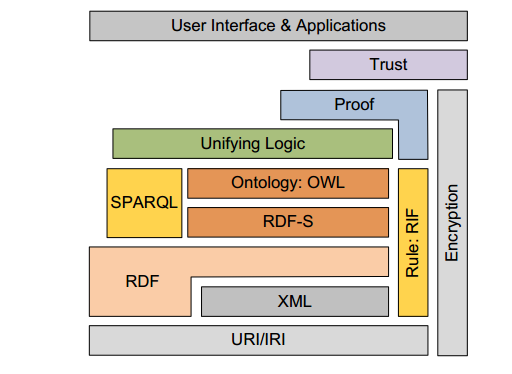
\includegraphics[width=1\textwidth]{Capture0}
\caption{Semantic web architecture}
\end{figure}
{  The first layer, URI and Unicode, follows the important features of the existing WWW. Unicode is a standard of encoding international character sets and it allows that all human languages can be used (written and read) on the web using one standardized form. Uniform Resource Identifier (URI) is a string of a standardized form that allows to uniquely identify resources (e.g., documents). A subset of URI is Uniform Resource Locator (URL), which contains access mechanism and a (network) location of a document - such as http://www.example.org/. Another subset of URI is URN that allows to identify a resource without implying its location and means of dereferencing it - an example is urn:isbn:0-123-45678-9. The usage of URI is important for a distributed internet system as it provides understandable identification of all resources. An international variant to URI is Internationalized Resource Identifier (IRI) that allows usage of Unicode characters in identifier and for which a mapping to URI is defined. In the rest of this text, whenever URI is used, IRI can be used as well as a more general concept.Extensible Markup Language (XML) layer with XML namespace and XML schema definitions makes sure that there is a common syntax used in the semantic web. XML is a general purpose markup language for documents containing structured information. A XML document contains elements that can be nested and that may have attributes and content. XML namespaces allow to specify different markup vocabularies in one XML document. XML schema serves for expressing schema of a particular set of XML documents.A core data representation format for semantic web is Resource Description Framework (RDF). RDF is a framework for representing information about resources in a graph form. It was primarily intended for representing metadata about WWW resources, such as the title, author, and modification date of a Web page, but it can be used for storing any other data. It is based on triples subject-predicate-object that form graph of data. All data in the semantic web use RDF as the primary representation language. The normative syntax for serializing RDF is XML in the RDF/XML form. Formal semantics of RDF is defined as well.RDF itself serves as a description of a graph formed by triples. Anyone can define vocabulary of terms used for more detailed description. To allow standardized description of taxonomies and other ontological constructs, a RDF Schema (RDFS) was created together with its formal semantics within RDF. RDFS can be used to describe taxonomies of classes and properties and use them to create lightweight ontologies.
More detailed ontologies can be created with Web Ontology Language OWL. The OWL is a language derived from description logics, and offers more constructs over RDFS. It is syntactically embedded into RDF, so like RDFS, it provides additional standardized vocabulary. OWL comes in three species - OWL Lite for taxonomies and simple constrains, OWL DL for full description logic support, and OWL Full for maximum expressiveness and syntactic freedom of RDF. Since OWL is based on description logic, it is not surprising that a formal semantics is defined for this language.RDFS and OWL have semantics defined and this semantics can be used for reasoning within ontologies and knowledge bases described using these languages. To provide rules beyond the constructs available from these languages, rule languages are being standardized for the semantic web as well. Two standards are emerging - RIF and SWRL.For querying RDF data as well as RDFS and OWL ontologies with knowledge bases, a Simple Protocol and RDF Query Language (SPARQL) is available. SPARQL is SQL-like language, but uses RDF triples and resources for both matching part of the query and for returning results of the query. Since both RDFS and OWL are built on RDF, SPARQL can be used for querying ontologies and knowledge bases directly as well. Note that SPARQL is not only query language, it is also a protocol for accessing RDF data.}
\subsection{Resource Description framework}
{The Resource Description Framework 1 (RDF) is a language for representing information about resources in the World Wide Web. A resource is a physical or virtual entity, such as a personor an IP packet. RDF describes those resources in a subject-predicate-object structure.}
\subsubsection{Concept}
{RDF represents information by means of statements in a Subject-Predicate-Object structure:
\begin{enumerate}
\item {Subject: a resource that is described by the statement}
\item {Predicate: a property of the resource that is described}
\item {Object: the value of the property of the resource that is described}
\end{enumerate} 
{Take for example the statement “Abderrahmen's emailAdress is abderrahmen.sdiri@supcom.tn”. The parts are:
\begin{enumerate}
\item {Subject:Abderrahmen }
\item {Predicate:emailAdress}
\item {Object: abderrahmen.sdiri@supcom.tn}
\end{enumerate}
{Since RDF is meant to be machine-processable, evey resource has to be unique to avoid confusion. The Web offers URI references to deal with this problem. Subjects and predicates are resources, and thus are to be represented by a URI reference. Objects can be resources, though they also can be a literal, which is a non-decomposable object, like a string or a number}
\subsection{Representation}
{RDF has in fact an inherent graph based structure, which can be serialized using turte, RDF/XML and others. The next paragraphs introduce representations for a group of statements. Forsome representations, an example is given for “Abderrahmen is called Abderrahmen S and is 24 years old. Ahmed is his friend. The FOAF  ontology is used to describe these statements. Note that since URIs can be long, they can be shortened in a more clear notation, using prefixes. Therefore a URI reference is split up in a namespace and local name.
This namespace is represented by a prefix. The notation is shortened as  \verb!prefix:local_name!. For instance,\url{ http://xmlns.com/foaf/0.1/name}  is  equivalent to \verb!foaf:name!, using foaf as a prefix for  \url{http://xmlns.com/foaf/0.1/}.}
\subsubsection{Graph model notation}
{RDF statements lend themselves easily to be represented as a graph. Subjects and objects are the equivalent of the nodes and predicates are labeled edges. Conceptually this means that a subject is connected to an object by means of a predicate. The following graph is the
representation of the earlier given example. Note that every resource, used as a subject or object, is unique; per resource only one node exists.}
\subsubsection{Turtle}
{Turtle (Terse RDF Triple Language) is a format for expressing data in the Resource Description Framework (RDF) data model with a syntax similar to SPARQL. RDF, in turn, represents information using "triples", each of which consists of a subject, a predicate, and an object. Each of those items is expressed as a Web URI.Turtle provides a way to group three URIs to make a triple, and provides ways to abbreviate such information, for example by factoring out common portions of URIs. For example:\\
<http://example.org/person/Abderrahmen> <http://example.org/relation/student>  <http://example.org/engineeringSchools/SUP'COM> .}







\appendix

\section{Source Code}

\begin{lstlisting}
  print('Hello World!')
     use indentation and {special &characters}
\end{lstlisting}






\end{document}
